\chapter{Methodology and Implementation}
\label{chap:methodology}

Chapter~\ref{chap:problem} defined the formal CMDP governing telecom tower
energy management. This chapter presents the implemented solution
framework: the simulator and training pipeline (Sections~\ref{sec:overview}
and~\ref{sec:rationale}), the environment implementation
(Section~\ref{sec:env_impl}), the reward design and its justification
(Section~\ref{sec:reward_design}), the full comparison-policy set
(Section~\ref{sec:comparison_policies}), the experimental protocol
(Section~\ref{sec:evaluation_protocol}), \revised{and a summary of the implemented configuration and
scope limitations (Section~\ref{sec:impl_deviations}).}

% ============================================================
\section{Methodology Overview}
\label{sec:overview}
% ============================================================

Figure~\ref{fig:chapter_roadmap} orients the reader before the technical
detail that follows: the CMDP formulated in Chapter~\ref{chap:problem} is
solved by the RLInv agent designed in this chapter, trained and
evaluated as described here, with the resulting evidence reported in
Chapter~\ref{chap:results}.

\begin{figure}[htbp]
\centering
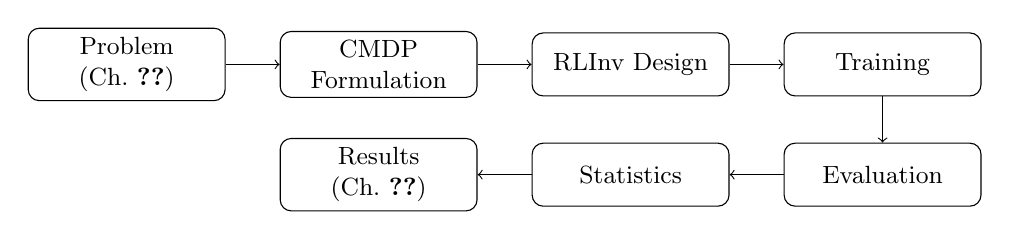
\begin{tikzpicture}[
  node distance=1.2cm,
  box/.style={draw, rounded corners, align=center,
              minimum width=2.5cm, minimum height=0.8cm,
              text width=2cm, 
              font=\small}
]

%% --- Row 1 ---
\node[box] (problem) {Problem (Ch.~\ref{chap:problem})};
\node[box, right of=problem, xshift=2cm] (cmdp)  {CMDP Formulation};
\node[box, right of=cmdp,    xshift=2cm] (rlinv) {RLInv Design};
\node[box, right of=rlinv,   xshift=2cm] (train) {Training};

%% --- Row 2 (right-to-left flow) ---
\node[box, below of=train,   yshift=-0.2cm] (eval)    {Evaluation};
\node[box, left of=eval,     xshift=-2cm] (stats)   {Statistics};
\node[box, left of=stats,    xshift=-2cm] (results) {Results (Ch.~\ref{chap:results})};

%% --- Row 1 arrows ---
\draw[->] (problem) -- (cmdp);
\draw[->] (cmdp)    -- (rlinv);
\draw[->] (rlinv)   -- (train);

%% --- Snake arrow: row 1 to row 2 ---
\draw[->] (train) -- (eval);

%% --- Row 2 arrows (right to left) ---
\draw[->] (eval)  -- (stats);
\draw[->] (stats) -- (results);

\end{tikzpicture}%
\caption{Chapter roadmap: from the formal problem to the reported evidence.}
\label{fig:chapter_roadmap}
\end{figure}



Figure~\ref{fig:workflow} shows the overall pipeline from raw data to
operational metrics. The ITU/Zindi dataset is loaded and split per site
into a 45-day training block and a 15-day test block. Each site's time
series drives a Gymnasium-compatible \texttt{TelecomEnv} simulator.
\texttt{MaskablePPO} agents are trained within this simulator, producing a
learned policy that is subsequently frozen and evaluated across all ten
sites under four delivery-logistics scenarios. Operational
metrics---primarily Expected Energy Not Served (EENS)---are computed from
the evaluation rollouts. Exploratory data analysis of the dataset is
presented in Chapter~\ref{chap:datasets-setup}.

\begin{figure}[htbp]
\centering
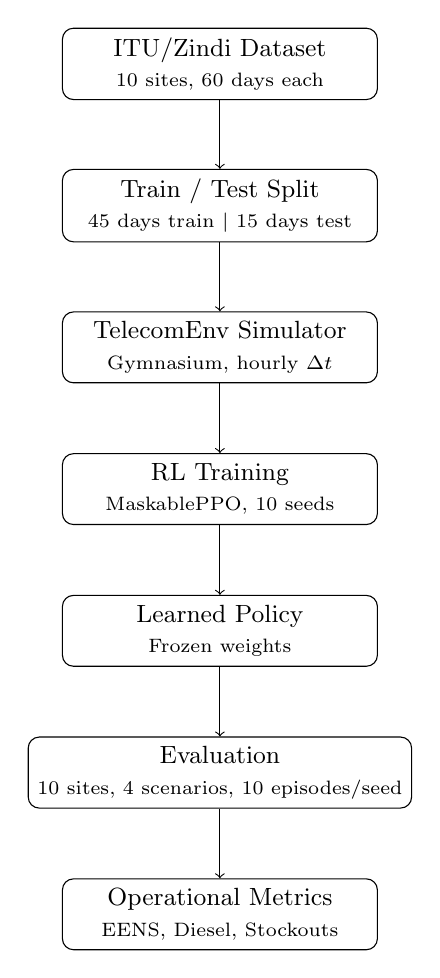
\begin{tikzpicture}[
  node distance=1.8cm,
  box/.style={draw, rounded corners, align=center,
              minimum width=4.0cm, minimum height=0.9cm, font=\small}
]
\node[box] (data)    {ITU/Zindi Dataset\\{\scriptsize 10 sites, 60 days each}};
\node[box, below of=data]   (split)   {Train / Test Split\\{\scriptsize 45 days train \textbar\ 15 days test}};
\node[box, below of=split]  (env)     {TelecomEnv Simulator\\{\scriptsize Gymnasium, hourly $\Delta t$}};
\node[box, below of=env]    (train)   {RL Training\\{\scriptsize MaskablePPO, 10 seeds}};
\node[box, below of=train]  (policy)  {Learned Policy\\{\scriptsize Frozen weights}};
\node[box, below of=policy] (eval)    {Evaluation\\{\scriptsize 10 sites, 4 scenarios, 10 episodes/seed}};
\node[box, below of=eval]   (metrics) {Operational Metrics\\{\scriptsize EENS, Diesel, Stockouts}};

\draw[->] (data)    -- (split);
\draw[->] (split)   -- (env);
\draw[->] (env)     -- (train);
\draw[->] (train)   -- (policy);
\draw[->] (policy)  -- (eval);
\draw[->] (eval)    -- (metrics);
\end{tikzpicture}
\caption{End-to-end workflow of the proposed reinforcement-learning
framework, from dataset ingestion through policy training to operational
evaluation.}
\label{fig:workflow}
\end{figure}



% ============================================================
\section{Design Decisions}
\label{sec:rationale}
% ============================================================

\subsection{Why PPO rather than value-based methods?}

\revised{PPO was initially selected for its clipped
policy updates and compatibility with feasibility
masking \citep{schulman2017proximal,perera2021application,
zhang2021deep}. DQN \citep{mnih2015humanlevel} and A2C
were subsequently evaluated as alternative reinforcement
learning methods. The resulting controller comparisons
are reported in Section~\ref{sec:g4_rl_comparison};
the initial algorithm choice is not treated as evidence
of PPO's superior reliability.}

\subsection{Why MaskablePPO rather than penalty-based constraint handling?}

Penalty-based constraint handling adds infeasibility costs to the reward.
A finite penalty cannot guarantee zero hard violations: if the coefficient
is poorly calibrated the policy still explores infeasible actions, and a
diesel stockout or battery deep-discharge causes an operational constraint
violation or loss of service. \texttt{MaskablePPO} from \texttt{sb3-contrib}
instead sets infeasible action logits to $-\infty$ before the softmax, making
the probability of any infeasible action exactly zero by construction. This
converts the constraint set $\mathcal{C}(s_t)$ into a hard structural
property of the policy distribution rather than something the policy must
learn to avoid; a violation-backstop coefficient ($\mu$) is still retained
(Section~\ref{sec:reward_design}) as a secondary safeguard. \revised{A7 is an unmasked PPO comparator.
Its historical training used a fixed initial-inventory
fraction of 0.60, whereas RLInv used a uniform
distribution over $[0.20,0.90]$. Consequently,
this comparison does not isolate the causal
effect of action masking
(Chapter~\ref{chap:results}).}

\subsection{Why a unified agent (RLInv) alongside decomposed control?}


Classical decomposed approaches use separate controllers
for inventory ordering and energy dispatch. These
decisions are coupled: generator operation depletes
diesel inventory, while available inventory constrains
generator dispatch. RLInv addresses both decisions
within one learned policy.

Two decomposed configurations provide comparisons.
TrackB combines an $(s,S)$ ordering rule with a
separately trained PPO dispatch controller. A6 uses
\revised{the same $(s,S)$ policy class} but retrains dispatch with
the full observation vector and a reduced two-action
space, compared with RLInv's six-action joint space.

These comparisons assess the implemented control
configurations. The action-space and observation
differences are documented alongside their results
in Chapter~\ref{chap:results}.


\subsection{Why a discrete action space?}

Although battery dispatch could be formulated as a continuous RL action,
rural charge-controllers follow fixed priority rules rather than
continuous analogue setpoints. The implemented system therefore delegates
battery dispatch to a deterministic priority rule, focusing RL learning
capacity on the logistics decisions (generator commitment and ordering)
where non-myopic planning is most valuable.

\subsection{Why a flat MLP rather than modular encoders?}


\revised{The implemented controller uses separate actor
and critic MLPs, each with two 256-unit hidden layers,
for the 11-dimensional observation.} Modular domain-specific encoders introduce
additional architectural hyperparameters (encoder depth, output dimension,
concatenation structure) whose benefits were not investigated in this work
given the small observation dimensionality. The flat design simplifies
implementation and is directly supported by the Stable-Baselines3
\texttt{MlpPolicy} without a custom feature extractor. 
The same hidden-layer configuration was used
for PPO-based policies unless otherwise stated;
observation dimensions and training conditions
could differ between controllers.

\revised{Table~\ref{tab:architecture} reports the implemented RLInv
architecture, comprising separate actor and critic networks with
Tanh activations and 139,527 trainable parameters in total.}

\begin{table}[htb]
\centering
\small
\caption{RLInv network architecture. Actor logits are masked
(Section~\ref{sec:rationale}) before the softmax; the critic head is
\revised{used during training but not for action selection at inference}.}
\label{tab:architecture}
\begin{tabular}{lll}
\toprule
\textbf{Layer} & \textbf{Shape} & \textbf{Parameters} \\
\midrule
Input (observation) & 11 & --- \\
\revised{Actor hidden layer 1 (Tanh)} & $11 \to 256$ & 3{,}072 \\
\revised{Actor hidden layer 2 (Tanh)} & $256 \to 256$ & 65{,}792 \\
Actor head (masked) & $256 \to 6$ & 1{,}542 \\
\revised{\textbf{Actor subtotal}} & & \revised{\textbf{70{,}406}} \\
\midrule
\revised{Critic hidden layer 1 (Tanh)} & $11 \to 256$ & \revised{3{,}072} \\
\revised{Critic hidden layer 2 (Tanh)} & $256 \to 256$ & \revised{65{,}792} \\
\revised{Critic value head} & $256 \to 1$ & 257 \\
\revised{\textbf{Critic subtotal}} & & \revised{\textbf{69{,}121}} \\
\midrule
\textbf{Total} & & \revised{\textbf{139{,}527}} \\
\bottomrule
\end{tabular}
\end{table}



% ============================================================
\section{Environment Implementation}
\label{sec:env_impl}
% ============================================================

\subsection{Structure and observation}

The environment is implemented as a Gymnasium-compatible class
\texttt{TelecomEnv} operating at hourly resolution ($\Delta t = 1$\,h)
with 720-step training episodes (30 simulated days) and 360-step
evaluation episodes (15 days, matching the held-out test split exactly).
During training, a random start index is sampled within the 45-day
training block; evaluation is fixed to the 15-day test block. Episodes
terminate after the fixed step count; no early termination condition is
used.

The 11-dimensional observation at each step is:
\begin{multline}
s_t = \bigl[
  \SoC_t,\;
  \Inv_t,\;
  \texttt{pending\_flag}_t,\;
  \texttt{pending\_qty}_t,\;
  P_t^{\PV},\; \\
  P_t^{\Load},\;
  G_t,\;
  \sin(2\pi h_t/24),\;
  \cos(2\pi h_t/24),\;
  \tau_t,\;
  H_t^{\mathrm{rem}}
\bigr].
\end{multline}
The pending-delivery state uses a binary flag (order in transit?) and a
scalar quantity (fuel expected on arrival), which together are logically
equivalent to the single pipeline scalar $\Pipe_t$ of
Chapter~\ref{chap:problem} under the single-outstanding-order constraint.
Two further channels complete the 11-dimensional vector. \texttt{hours\_since\_order\_n}
($\tau_t$) is the elapsed time since the last order was placed,
resetting to zero whenever a new order is issued; it is active in the
standard experiments. \texttt{delivery\_remaining\_n} ($H_t^{\mathrm{rem}}$) is present
in the observation vector but zero in the principal geometric,
no-ETA campaign reported throughout this thesis; it exists for
compatibility with a separate lognormal-forecast extension outside the
primary scope of this work. RLInv-DA (Chapter~\ref{chap:results})
additionally adds an EWMA delay estimate as a twelfth channel, producing
a 12-dimensional observation for that exploratory extension only.
Hour-of-day is encoded as sine--cosine features so that hours~23 and~0 are
adjacent in feature space. \revised{Grid availability is exogenous: the principal evaluation uses
the recorded site series, while a separate robustness experiment
samples grid outages from a fitted stochastic model.} All continuous features are normalised online using
\texttt{VecNormalize}; statistics are frozen before evaluation.

\subsection{Action space, battery rule, and inventory}

Diesel inventory is tracked in kWh-equivalent units. Tank capacity is
$C^{\Tank} = 72\,\bar{D}$, \revised{where $\bar{D}$ is the mean
hourly load of the data segment supplied to the simulator.
The same mean load is used for reward normalisation, with both
quantities calculated separately for training and evaluation.}

A generator start is permitted only if
$\Inv_t \geq 1.20 \times P_{\mathrm{rated}}^{\DG} \times 2\,\mathrm{h}$,
\revised{providing a startup fuel reserve equivalent to two hours
of rated generator output with a 20\% safety margin.}

The action space is discrete with six elements encoding
$\DG_t \in \{0,1\}$ and $Q_t \in \{0,\;0.30\,C^{\Tank},\;0.60\,C^{\Tank}\}$
--- order quantities are expressed as a percentage of tank capacity rather
than a fixed litre value, so that the same action encoding applies
consistently across sites of different sizes.

Battery
dispatch is not a learnable action; it is determined by a fixed
energy-priority rule inside the simulator:
\[
\text{PV} \;\to\; \text{Grid} \;\to\; \text{Battery discharge}
\;\to\; \text{DG} \;\to\; \text{Unmet load.}
\]

\revised{The battery update uses charge and discharge
coefficients of 0.35 and 1.20, respectively, as provided
in the site data (Eq.~\eqref{eq:soc}).}

Diesel delivery delay is modelled as a geometric process: once an order is
placed, delivery occurs at each subsequent step with a fixed per-step
probability $p$, giving a mean lead time of $1/p$ hours. The geometric
model preserves a Markovian state with only the two pending-order scalars
(flag and quantity), avoiding a countdown vector. Four scenarios are used
in the evaluation campaign: Normal ($p=1/24$, mean 24\,h), Delayed
($p=1/48$, mean 48\,h), Monsoon ($p=1/72$, mean 72\,h), and Extreme
($p=1/336$, mean 336\,h). The learned policies in the primary
comparison---RLInv, TrackB, A5, A6, and A7---were trained under Normal
logistics. All nine policies were then evaluated under Normal, Delayed,
Monsoon, and Extreme conditions.
Each scenario represents a distinct operating regime rather than an
arbitrary parameter value (Table~\ref{tab:scenario_meaning}).
The complete experimental protocol is presented in
Chapter~\ref{chap:experimental-execution}, including the use of ten
sites, ten independent training seeds, and all evaluation scenarios.

\begin{table}[htb]
\centering
\small
\caption{Operational interpretation of the four evaluation scenarios.}
\label{tab:scenario_meaning}
\begin{tabular}{lp{7.5cm}}
\toprule
\textbf{Scenario} & \textbf{Represents} \\
\midrule
Normal   & Routine logistics with nominal supplier performance \\
Delayed  & Moderate but recurring delivery disruption \\
Monsoon  & Seasonal degradation with prolonged uncertainty \\
Extreme  & Severe logistics stress approaching worst-case operating
           conditions \\
\bottomrule
\end{tabular}
\end{table}

Several candidate lead-time parameterisations were explored during
simulator calibration. The four scenarios span routine operation through
severe logistics disruption. Intermediate lead-time settings explored
during calibration produced similar trends and were omitted to keep the
final design interpretable and non-redundant.

\subsection{Safety handling}

\revised{For MaskablePPO controllers, feasibility masks
are applied before action sampling. The simulator also
blocks or clips infeasible requests, including those
submitted by unmasked controllers. The following two
rules govern DG activation and replenishment feasibility.}

\begin{enumerate}
  \item \textbf{DG masking:} all actions with $\DG_t = 1$ are disabled if
inventory is below the \revised{minimum startup fuel threshold}.
  \item \textbf{Order masking:} all non-zero order actions are disabled if
  a delivery is already pending, enforcing the single-outstanding-order
  constraint. Order quantities exceeding remaining tank headroom are also
  clipped.
\end{enumerate}

\texttt{MaskablePPO} applies the mask by setting infeasible logits to
$-\infty$ before the softmax; the no-operation action is always feasible
as a safe fallback. Post-step physical clipping (SoC and inventory to
their bounds) provides a numerical backstop and contributes a small
penalty term to the reward (Section~\ref{sec:reward_design}). No adaptive Lagrangian update was implemented.

\revised{The archived A6--TrackB comparison records lower
EENS for A6 under Monsoon and Extreme logistics.
These controllers differ in masking, observation design
and combined-action handling. Under Extreme logistics,
their analytical reorder calibration also differs.
The separate RLInv--A7 comparison finds no statistically
significant mean-EENS difference
(Chapter~\ref{chap:results}).}


\subsection{Agent architecture and training}

Figure~\ref{fig:rlinv_loop} illustrates the RLInv
decision loop: \revised{the policy computes action
logits, applies feasibility masking and samples an
action. The environment then advances and computes
a reward. PPO updates the policy after collecting
training rollouts.}

\begin{figure}[htbp]
\centering
\begin{tikzpicture}[
  node distance=1.6cm,
  box/.style={draw, rounded corners, align=center,
              minimum width=3.2cm, minimum height=0.8cm, font=\small},
  >=Stealth
]
\node[box] (order)
  {\revised{Policy computes}\\\revised{action logits}};
\node[box, right=of order] (mask)
  {\revised{Mask and}\\\revised{sample action}};
\node[box, right=of mask]    (env)   {Environment step};
\node[box, below=of env]     (reward) {Reward computed};
\node[box, left=of reward]   (ppo)    {PPO update};
\node[box, left=of ppo]      (policy) {Policy updated};

\draw[->] (order)  -- (mask);
\draw[->] (mask)   -- (env);
\draw[->] (env)    -- (reward);
\draw[->] (reward) -- (ppo);
\draw[->] (ppo)    -- (policy);
\draw[->] (policy.north) -- (order.south);
\end{tikzpicture}
\caption{RLInv's per-step decision loop. The mask is applied before
sampling, so infeasible actions have zero probability rather than being
sampled and penalised after the fact; PPO's policy update closes the
loop over the course of training.}
\label{fig:rlinv_loop}
\end{figure}

RLInv uses \texttt{MaskablePPO} with a flat MLP $[256,\,256]$ policy.
Training used four parallel \texttt{SubprocVecEnv} environments for
400{,}000 timesteps per seed. Ten independent training seeds were used
to reduce sensitivity to stochastic policy optimisation and to enable
paired statistical comparisons across identical site--scenario
combinations: (42, 123, 777, 7, 13, 21, 99, 314, 500, 999). The first
three (42, 123, 777) were retained from Phase~2 and the
remaining seven were added to increase statistical power for the
seed-level paired comparisons reported in Chapter~\ref{chap:results}. A custom evaluation callback synchronised
\texttt{VecNormalize} statistics between the training and evaluation
environments before each validation pass, preventing observation-scale
mismatch. Training inventory was randomised over $[0.20,\,0.90]\,C^{\Tank}$
\revised{to expose the policy to varying initial fuel levels;}
evaluation randomises initial inventory over $[0.3,\,0.9]\,C^{\Tank}$.

A convergence check extended training to 560{,}000 steps on three
representative sites (1, 5, and~7) using seed~42. Sites~1 and~7 showed no
change in evaluation reward beyond 400{,}000 steps, indicating early
convergence. Site~5 exhibited high reward variance across independent
runs regardless of step count, consistent with its classification as a
grid-constrained site. The 400{,}000-step checkpoint was therefore
retained for all sites and seeds.

Table~\ref{tab:hyperparams} lists all training hyperparameters.

\begin{table}[htb]
\centering
\small
\caption{\revised{PPO-family training configuration.
RLInv, A5 and A6 use MaskablePPO; TrackB and A7
use standard PPO.}}
\label{tab:hyperparams}
\begin{tabular}{p{3.8cm}p{4.8cm}p{4.4cm}}
\toprule
\textbf{Parameter} & \textbf{Value} & \textbf{Rationale} \\
\midrule
Algorithm &
\revised{MaskablePPO (RLInv/A5/A6); PPO (TrackB/A7)} &
\revised{Pre-action masking for MaskablePPO only} \\
Policy network
  & \revised{Separate actor and critic MLPs $[256,\,256]$, Tanh}
  & CPU-feasible capacity \\
Total timesteps        & 400{,}000 per seed                 & Fixed training budget used consistently across all runs \\
Learning rate          & $3\times10^{-4}$ (linear decay)    & PPO standard \\
Clip ratio $\epsilon$  & 0.2                                & PPO standard \\
Entropy coefficient    & 0.01                               & Encourage exploration \\
Discount $\gamma$      & 0.99                               & Effective horizon $\approx$\,100\,h; see Chapter~\ref{chap:results} for a discount-factor sensitivity check against $\gamma=0.995$ \\
GAE $\lambda$          & 0.95                               & Bias--variance balance \\
$n_{\text{steps}}$     & 2048                               & Rollout buffer length \\
Batch size             & 256                                & CPU-friendly mini-batch \\
$n_{\text{epochs}}$    & 10                                 & PPO inner loop \\
Parallel environments  & 4 (\texttt{SubprocVecEnv})         & CPU parallelism; reduced from 8 due to OS process handle limits \\
Seeds                  & 42, 123, 777, 7, 13, 21, 99, 314, 500, 999 & \revised{Ten training seeds for the original
policy and ablation comparisons}\\
\bottomrule
\end{tabular}
\end{table}


% ============================================================
\section{Reward Design}
\label{sec:reward_design}
% ============================================================

The reward is a shaped, normalised scalar designed to penalise
unreliability far more heavily than fuel cost:
\[
r_t =
-\alpha \dfrac{E_t^{\DG}}{\bar{D}}
-\beta  \dfrac{E_t^{\Grid}}{\bar{D}}
-\lambda \dfrac{U_t}{\bar{D}}
-\gamma_r\,\mathbb{I}\!\bigl[U_t>0 \wedge \Inv_t^{\mathrm{postDG}}=0\bigr]
-\mu\,V_t,
\]
where $E_t^{\DG}$ is diesel energy consumed, $E_t^{\Grid}$ is grid energy
drawn, $U_t$ is unmet load energy (kWh), $\mathbb{I}[\cdot]$ is a cliff
penalty triggered by a stockout coinciding with an active load shortfall,
and $V_t$ indicates a physical-clipping event (SoC or inventory bound
violation caught by the post-step numerical backstop). Dividing all
energy terms by the site mean hourly load $\bar{D}$ normalises the signal
to a comparable scale across sites of different size. \revised{Here $\Inv_t^{\mathrm{postDG}}$ denotes on-site fuel
remaining after generator dispatch and before any pending delivery is
processed. The stockout flag is raised when this quantity is zero
and unmet load is positive.}

\revised{This is the implemented objective defined in
Chapter~\ref{chap:problem}, with reward equal to negative step cost.
Order-placement, ordered-volume, inventory-holding,
battery-degradation and carbon costs are not explicit terms.}

\textbf{Note on notation.} The stockout-cliff coefficient $\gamma_r$ is
unrelated to the PPO discount factor $\gamma$ used elsewhere in this
chapter; the subscript distinguishes them.

\subsection{Coefficient values and justification}

The default coefficients are $\alpha=1.0$, $\beta=0.4$, $\lambda=100$,
$\gamma_r=200$, $\mu=20$. Each is chosen for a specific, stated reason
rather than by unconstrained tuning:

\begin{itemize}
\item \textbf{$\lambda = 100$} (unmet-load penalty) assigns unmet energy
a substantially larger penalty than diesel use, reflecting that one
kWh of unserved telecom load is far more costly operationally than one
kWh of diesel-generated energy at the most constrained site in the
dataset (site~5). This large ratio is the mechanism by which the reward
prioritises reliability over fuel economy.
\item \textbf{$\gamma_r = 200$} (stockout cliff) is set to exactly twice
$\lambda$, reflecting that a stockout coinciding with unmet load is a
qualitatively different failure mode from unmet load alone (a hard
reliability failure, not merely a cost), and should be penalised more
severely rather than merely proportionally.
\item \textbf{$\beta = 0.4$} (grid-energy weight)
\revised{assigns a lower reward penalty to grid consumption
than to diesel generation. Grid allocation follows the
simulator's fixed energy-priority rule.}
\item \textbf{$\mu = 20$} (physical-violation penalty) is deliberately
small: it is a numerical backstop for the rare event that hard masking
still allows a boundary violation (e.g.\ through clipping), not a primary
control lever. Its sensitivity is tested directly in
Chapter~\ref{chap:results}, where broad coefficient ranges are evaluated
across all principal reward parameters, with full values reported there.
\end{itemize}

The selected coefficients encode engineering design preferences rather
than uniquely optimal values, guided by the engineering rationale
discussed below and by prior work
\citep{hu2024performance}. Chapter~\ref{chap:results} evaluates RLInv's
own performance across broad coefficient ranges, including a 20-fold
range for $\lambda$, to assess the sensitivity of RLInv's performance to
these choices.


% ============================================================
\section{Comparison Policies}
\label{sec:comparison_policies}
% ============================================================


The original evaluation comprised six primary
comparison policies and three targeted ablations.
Table~\ref{tab:ablation-design} maps every policy to the architectural
question it addresses; Figure~\ref{fig:rlinv_trackb} contrasts the two
principal control architectures directly.

\begin{figure}[htbp]
\centering
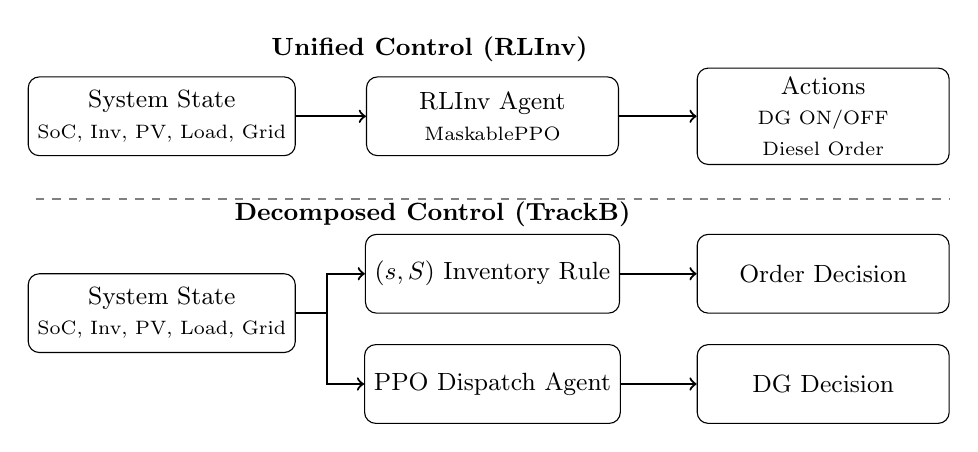
\begin{tikzpicture}[
  box/.style={draw, rounded corners=4pt, align=center,
              minimum width=3.2cm, minimum height=1.0cm, font=\small},
  arrow/.style={->, thick},
  label/.style={font=\small\bfseries}
]
\node[label] at (3.4, 0.85) {Unified Control (RLInv)};
\node[box] (state1) at (0, 0)
  {System State\\{\scriptsize SoC, Inv, PV, Load, Grid}};
\node[box] (agent1) at (4.2, 0)
  {RLInv Agent\\{\scriptsize MaskablePPO}};
\node[box] (acts1) at (8.4, 0)
  {Actions\\{\scriptsize DG ON/OFF}\\{\scriptsize Diesel Order}};
\draw[arrow] (state1) -- (agent1);
\draw[arrow] (agent1) -- (acts1);
\draw[dashed, gray] (-1.6, -1.05) -- (10.0, -1.05);

\node[label, anchor=west] at (0.8, -1.25) {Decomposed Control (TrackB)};
\node[box] (state2) at (0, -2.5)
  {System State\\{\scriptsize SoC, Inv, PV, Load, Grid}};
\node[box] (ss)       at (4.2, -2.0) {$(s,S)$ Inventory Rule};
\node[box] (order2)   at (8.4, -2.0) {Order Decision};
\node[box] (dispatch) at (4.2, -3.4) {PPO Dispatch Agent};
\node[box] (dg2)      at (8.4, -3.4) {DG Decision};
\draw[arrow] (state2.east) -- ++(0.4,0) |- (ss.west);
\draw[arrow] (state2.east) -- ++(0.4,0) |- (dispatch.west);
\draw[arrow] (ss)       -- (order2);
\draw[arrow] (dispatch) -- (dg2);
\end{tikzpicture}
\caption{Structural comparison of the two principal control
architectures. RLInv jointly optimises generator dispatch and diesel
ordering within a single reinforcement-learning policy. TrackB separates
the two decisions: a classical $(s,S)$ rule handles ordering while a PPO
agent handles dispatch.}
\label{fig:rlinv_trackb}
\end{figure}

\textbf{RLInv} is the proposed unified controller: \texttt{MaskablePPO}
learns to select generator commitment and diesel order quantity jointly
at each step, with all masking rules active.

\textbf{TrackB} is the decomposed-control comparison: a calibrated $(s,S)$
inventory rule determines ordering, while a PPO dispatch agent controls
the generator using the same hidden-layer architecture ($[256,\,256]$
MLP) as RLInv. The dispatch agent's input is a reduced 6-dimensional
observation (state-of-charge, PV, load, grid, and the two cyclic
hour-of-day features only; inventory-related dimensions are withheld
since ordering is handled externally), so "identical network" refers to
matched hidden-layer capacity, not an identical input layer; this keeps
the comparison focused on control structure rather than a confound from
network size.
\revised{\textbf{TrackB implementation limitation.}
Source inspection identified a combined-action fallback in the
original TrackB wrapper. When the requested generator--order
combination is infeasible, the wrapper replaces the entire
action with index zero (DG off, no order). This can cancel
an otherwise feasible generator or ordering decision.
The frequency and effect of this behaviour in the archived
runs have not been established. TrackB is therefore retained
as an archived configuration comparison, not as an isolated
test of masking or dispatch architecture.}
\begin{quote}
\textbf{Implementation Note.} The reorder point covers estimated mean
consumption over the expected delivery lead time, subject to lower and
upper clipping limits:
$s_{\mathrm{norm}} = \mathrm{clip}(k_s \cdot \bar{D} \cdot \mathbb{E}[L]
\,/\, C^{\Tank},\, 0.05,\,0.95)$ with safety multiplier $k_s=1$, and
order-up-to level $S_{\mathrm{norm}} = \mathrm{clip}(0.85,\,
s_{\mathrm{norm}}+0.10,\,0.95)$. \revised{The analytical rule is instantiated separately in
TrackB and A6, subject to the Extreme-scenario calibration
limitation discussed below. B1, MPC and Oracle-MPC use fixed
thresholds of $s=0.25$ and $S=0.85$.}
\end{quote}

\revised{\textbf{MPC} combines default $(s,S)$ ordering
with a receding-horizon mixed-integer linear programme
solved using HiGHS (\texttt{scipy.optimize.milp}).
The planning horizon is 24 hours. Load and solar
generation use persistence forecasts, while future grid
availability is read from the recorded site trace when
available. The MILP contains 24 generator and 24 grid
binary variables, together with continuous energy and
state variables.

The MILP plans battery and generator dispatch, but only
the generator commitment and classical ordering decision
are submitted to the environment. Actual battery dispatch
continues to follow the simulator's fixed priority rule.
The MPC therefore has additional grid information and
a planning model that differs from executed dispatch.
Its 24-hour horizon is shorter than the 336-hour mean
delivery time under Extreme logistics.} A
third variant using a learned 24-hour forecasting module in place of the
persistence forecast was also implemented and evaluated during
development; it is not part of the primary comparison, as it did not
alter the qualitative conclusions drawn from the persistence-forecast
MPC baseline.


\textbf{Oracle-MPC} uses the realised future load, solar-generation and
grid-availability traces over the remaining evaluation horizon (perfect
information) rather than a persistence estimate, and its planning
horizon extends to the full 360-step evaluation episode rather than 24
hours. Diesel ordering remains governed by the \revised{default} $(s,S)$ rule, and
delivery timing remains stochastic.
\revised{Oracle-MPC serves as a perfect-information
dispatch reference. The comparison with RLInv
retains the documented differences in
replenishment and dispatch configurations.}


\textbf{B0} is a rule-based heuristic: a fixed-threshold inventory
policy using uncalibrated inventory thresholds, paired with threshold
dispatch, requiring no training. \revised{\textbf{B1} uses fixed $(s,S)$ ordering thresholds
($s=0.25$, $S=0.85$) and follows a generator-dispatch rule
similar to B0, with a default SoC threshold of 0.25
compared with 0.15 in B0.}

\textbf{A7} is vanilla PPO trained without action masking and serves as an
unmasked comparator.

\revised{\textbf{A5} retains the 11-dimensional observation
interface but zeros five logistics-related channels:
inventory level, pending-order flag, pending quantity,
elapsed time since ordering, and remaining delivery time.
The other six channels remain available. The A5 training
script permits initial-inventory settings different from
RLInv's $[0.20,0.90]$ training range; the exact historical
A5 invocation has not been independently verified.
Accordingly, the archived comparison does not isolate
the causal effect of inventory observability.}

\textbf{A6} provides a cleaner ordering ablation while acknowledging
that the dispatch policy is re-learned under a reduced action space,
rather than a perfectly controlled isolation of the ordering decision
alone. In
this variant the RL agent controls only generator commitment under a
reduced \texttt{Discrete(2)} action space, while diesel ordering is
\revised{handled by a separately instantiated analytical
$(s,S)$ rule from the same policy class as TrackB.} The observation space, reward function, and environment
dynamics remain identical to RLInv. Because the dispatch policy is
re-learned under the smaller action space, A6 provides a cleaner ordering
ablation than TrackB, which confounds ordering mechanism and dispatch
architecture simultaneously; both comparisons are reported in
Chapter~\ref{chap:results} for this reason.
\revised{\textbf{A6--TrackB calibration limitation.}
Both controllers were trained under Normal logistics
and evaluated under the four delivery scenarios.
During evaluation, TrackB constructs its classical
ordering rule using the selected scenario's lead-time
parameter. The current A6 factory does not explicitly
map Extreme logistics and instead uses the Normal
lead-time parameter for its analytical reorder threshold.
Consequently, the two controllers cannot be assumed
to use identical ordering thresholds under Extreme
logistics. The effect of this difference on the
archived EENS results has not been independently quantified.}

\begin{table}[htb]
\centering
\small
\caption{Policies evaluated in the experimental campaign,
their control mechanisms, and the question each addresses.}
\label{tab:ablation-design}
\begin{tabularx}{\textwidth}{
    >{\raggedright\arraybackslash}p{1.4cm}
    >{\raggedright\arraybackslash}p{2.15cm}
    >{\raggedright\arraybackslash}p{2.25cm}
    >{\raggedright\arraybackslash}p{2.0cm}
    >{\raggedright\arraybackslash}X
}
\toprule
\textbf{Label} &
\textbf{Ordering} &
\textbf{Dispatch} &
\textbf{Forecast} &
\textbf{Primary question} \\
\midrule
B0 &
Fixed threshold (uncalibrated) &
Threshold rule &
--- &
Baseline anchor \\
B1 &
$(s,S)$ rule &
Threshold rule &
--- &
\revised{Classical $(s,S)$ baseline} \\
MPC &
$(s,S)$ rule &
MILP, $H{=}24$ &
\revised{Load/PV persistence; grid look-ahead} &
Does optimal-but-myopic dispatch close the gap? \\
Oracle-MPC &
$(s,S)$ rule &
MILP, $H{=}360$ &
Perfect &
\revised{Perfect-information dispatch reference}\\
TrackB &
$(s,S)$ rule &
Learned (PPO) &
--- &
Joint vs.\ decomposed (H1, confounded) \\
A6 &
$(s,S)$ rule &
Learned (PPO, Discrete(2)) &
--- &
Joint vs.\ decomposed (H1, cleaner) \\
A7 &
Learned (joint) &
Learned (PPO, no mask) &
--- &
Action masking (H2) \\
A5 &
Learned (joint, no inv.\ obs.) &
Learned (PPO) &
--- &
Inventory observability (H3) \\
RLInv &
Learned (joint) &
Learned (PPO) &
--- &
Proposed system \\
\bottomrule
\end{tabularx}
\end{table}


\begin{table}[htbp]
\centering
\footnotesize
\setlength{\tabcolsep}{4pt}
\renewcommand{\arraystretch}{1.18}
\caption{\revised{Controller comparison groups,
information access, calibration and interpretation scope.}}
\label{tab:comparison_fairness}
\begin{tabularx}{\textwidth}{
p{2.1cm}
p{3.1cm}
p{3.1cm}
X
}
\toprule
\textbf{Group} &
\textbf{Information access} &
\textbf{Training or calibration} &
\textbf{Comparison scope} \\
\midrule

Original B0/B1 &
Current system observations &
Fixed heuristic thresholds &
Original rule-based reference configurations \\

MPC / Oracle-MPC &
Persistence forecasts / realised future energy traces &
MILP dispatch; default $(s,S)$ ordering &
Dispatch references with different forecast information
and planning horizons \\

Original RL controllers &
Site-specific training observations &
Ten training seeds; nominal 400k steps per run &
Original configuration and ablation comparisons;
action and observation spaces differ \\

Calibrated classical B1 variants &
Site-specific days 1--45 &
Analytic thresholds or training-window
$(s,S)$ calibration &
Held-out classical comparison;
training and tuning procedures differ \\

Supplementary null controllers &
Current simulator state and feasible actions &
Fixed non-learning decision rules &
Tests whether learning provides an incremental
advantage under the evaluated objective \\

Four-algorithm RL comparison &
Site-specific training observations &
Five training seeds; nominal 400k steps;
training initialisation differs &
Matched held-out evaluation;
not an isolated algorithm comparison \\

Shared RLInv / source-calibrated B1 &
Five source sites only &
Shared training or source-only threshold calibration &
Held-out-site comparison with source-data access
restricted to the same sites; compute differs \\

Target-site adaptation &
Source-pretrained policy or target-site training data &
50k/100k target interactions, with or without
source pretraining &
Adaptation comparison; total prior training
exposure differs \\

\bottomrule
\end{tabularx}
\end{table}

% ============================================================
\section{Experimental Protocol}
\label{sec:evaluation_protocol}
% ============================================================
This section specifies the experimental protocol required to reproduce
the evaluation, including training, testing, ablation, robustness, and
statistical comparison procedures. The quantitative results obtained
using this protocol are presented separately in
Chapter~\ref{chap:results}.

Figure~\ref{fig:eval_flow} summarises the overall protocol: policies are
trained, then evaluated on the held-out test window, with ablations and
sensitivity checks run against the same evaluation grid before the
paired statistical analysis is applied.

\begin{figure}[htbp]
\centering
\begin{tikzpicture}[
  node distance=1.2cm,
  box/.style={draw, rounded corners, align=center,
              minimum width=4.4cm, minimum height=0.8cm, font=\small}
]
\node[box] (train)      {Training (10 sites $\times$ 10 seeds)};
\node[box, below=of train]      (evaluate)  {Evaluation (4 scenarios, 10 episodes/seed)};
\node[box, below=of evaluate]   (ablations) {Ablations (A5, A6, A7 vs.\ RLInv)};
\node[box, below=of ablations]  (sensitivity) {Sensitivity checks (reward, tank,
                                                distribution, grid)};
\node[box, below=of sensitivity] (statistics) {Paired statistics (Chapter~\ref{chap:results})};

\draw[->] (train)      -- (evaluate);
\draw[->] (evaluate)   -- (ablations);
\draw[->] (ablations)  -- (sensitivity);
\draw[->] (sensitivity)-- (statistics);
\end{tikzpicture}
\caption{Overall evaluation protocol, from training through to the
paired statistical analysis reported in Chapter~\ref{chap:results}.}
\label{fig:eval_flow}
\end{figure}

All nine policies are evaluated on the 15-day held-out test window (days
46--60) of each of the ten ITU/Zindi sites, under all four delivery
logistics scenarios (Normal, Delayed, Monsoon, Extreme; defined in
Section~\ref{sec:env_impl}), with 10 episodes per seed and initial
inventory randomised uniformly over $[0.3,\,0.9]\,C^{\Tank}$. This is a
full factorial design: every policy is evaluated under every scenario at
every site, rather than the scenario coverage being policy-specific.
Table~\ref{tab:protocol_summary} summarises the evaluation grid at a
glance.

\begin{table}[htb]
\centering
\small
\caption{Experimental protocol at a glance.}
\label{tab:protocol_summary}
\begin{tabular}{lp{10.5cm}}
\toprule
\textbf{Item} & \textbf{Value} \\
\midrule
Sites                & 10 (all ITU/Zindi sites) \\
Seeds & 10 (42, 123, 777, 7, 13, 21, 99, 314, 500, 999) \\
Evaluation episodes  & 10 per seed \\
Scenarios            & 4 (Normal, Delayed, Monsoon, Extreme) \\
Policies evaluated   & 9 (B0, B1, MPC, Oracle-MPC, TrackB, A5, A6, A7, RLInv) \\
Primary metric       & EENS (kWh per episode) \\
Secondary metrics    & Diesel consumption, stockout events, orders placed, inventory trajectory \\
Statistical unit &
\revised{Paired seed means for original H1--H3 tests;
paired site means for expanded cross-site inference}
\\

\bottomrule
\end{tabular}
\end{table}

The evaluation archive also contains results for
two additional variants, \texttt{multi} and
\texttt{mpc\_forecast}.
The statistical units used for the different
comparisons are detailed in
Section~\ref{sec:metrics}.
\revised{The original controller comparisons use ten
training seeds. The extended four-algorithm study uses
five seeds, while cross-site generalisation uses three.
Non-learning policies have evaluation seeds but no
independently trained policy checkpoints. These cohorts
are analysed separately and are not treated as one
uniform training population.}
A subset of three sites (site2, site5, site7) is
additionally used for finer-grained robustness checks in
Chapter~\ref{chap:results} where a smaller, more tractable evaluation
grid is needed (e.g.\ reward and tank-capacity sensitivity sweeps); this
three-site subset was selected for load/solar/outage diversity and is
distinct from the site difficulty classification of
Chapter~\ref{chap:datasets-setup}, where only site2 and site5 are
classified Hard.

Full numerical results, including the primary comparison, the three
hypothesis tests, behavioural analysis, and all robustness checks
(reward weighting, discount factor, tank capacity, delivery-distribution
form, stochastic grid outages, and the RLInv-DA exploratory extension),
are reported in Chapter~\ref{chap:results}. All reported
experiments used ten evaluation episodes per seed. Within each
evaluation episode, stochastic delivery delays were independently
sampled according to the selected lead-time distribution while
maintaining the same underlying outage and demand profiles; different
random seeds therefore generated different delivery-delay realisations
under identical experimental settings.


% ============================================================
% Do not use \revised in the PDF string argument of \texorpdfstring
\section{\texorpdfstring{\revised{Implemented Configuration and Scope}}{Implemented Configuration and Scope}}
\label{sec:impl_deviations}

\subsection{\texorpdfstring{\revised{Configuration and modelling limits}}{Configuration and modelling limits}}
\label{sec:deviations_table}

\begin{revisedblock}
Table~\ref{tab:deviations} consolidates the implemented
controller and the modelling limits relevant to interpreting
the results. Earlier design choices are not treated as
features of the implemented model.
\end{revisedblock}
\begin{table}[htbp]
\centering
\scriptsize
\setlength{\tabcolsep}{4pt}
\ifshowrevisions\color{P3Rcolor}\fi
\caption{Implemented control design and limitations.}
\label{tab:deviations}
\begin{tabularx}{\textwidth}{p{2.3cm}X X}
\toprule
\textbf{Aspect} & \textbf{Implemented configuration} & \textbf{Scope or limitation} \\
\midrule
Control actions
& Six DG ON/OFF and tank-relative ordering combinations
& No continuous battery action or fixed-litre ordering \\[3pt]
Battery dispatch
& Fixed PV--grid--battery--DG supply priority
& Not jointly learned or economically co-optimised \\[3pt]
Inventory and orders
& kWh-equivalent fuel stock; one pending order; geometric lead times in main campaign
& Supplier delivery observations are simulated \\[3pt]
DG constraint
& Fuel-start reserve of 2.4 rated-output hours
& No enforced two-hour continuous ON-time \\[3pt]
Discount
& $\gamma=0.99$
& A 336-step-delayed outcome has weight about $0.034$ \\[3pt]
Reward
& Normalised diesel, grid and unmet-load penalties plus stockout and violation indicators
& No explicit order-placement, volume, holding, degradation or carbon costs; unmet load has weight $\lambda=100$ \\[3pt]
Action feasibility
& Action masking with simulator blocking and clipping
& No Lagrangian or learned recovery controller \\[3pt]
Battery coefficients
& Site-data charge/discharge coefficients; implemented discharge uses division by the coefficient
& Coefficients do not all follow conventional physical-efficiency interpretation \\[3pt]
Tank and scaling
& $C^{\Tank}=72\bar D$; $\bar D$ is computed from the supplied data slice
& Training and evaluation may use different $\bar D$ values \\[3pt]
Network and budget
& Separate actor and critic MLPs with $[256,256]$ hidden layers; nominal 400k training steps
& Actual PPO rollout-aligned count can exceed nominal budget \\
\bottomrule
\end{tabularx}
\end{table}

\subsection{Diesel supply-chain scope and assumptions}
\label{sec:supply_chain_scope}

This study models the diesel supply chain using the following
assumptions and scope boundaries, consolidated here for clarity, with
the corresponding formulation and implementation details presented in
Chapter~\ref{chap:problem} and Table~\ref{tab:deviations} above.

\textbf{Single vendor, single outstanding order.} The simulator models
one delivery pipeline per site with at most one order in transit at a
time; multi-vendor sourcing, vendor selection, and contractual or
pricing considerations are not represented. This keeps the pending-order
state a two-scalar quantity (Section~\ref{sec:env_impl}) rather than
requiring a general queue.

\textbf{Delivery delay as a stochastic process, not a routing problem.}
Delay is modelled as a per-site geometric (or, for robustness,
lognormal/Weibull) random process calibrated to a mean lead time, not as
the output of an explicit vehicle-routing, road-network, or
depot-inventory simulation. This is a deliberate abstraction: it
represents the \emph{effect} of upstream logistics uncertainty on a
single tower's replenishment decisions without requiring a full
logistics network model, which would require a fundamentally different
problem formulation centred on inventory-routing optimisation rather
than single-site inventory-aware control.

\textbf{Single-tower scope.}
Each evaluation episode controls one tower independently.
The shared-policy experiments train on multiple sites
but do not jointly control their operation. Shared
supplier capacity, delivery-slot competition and
fleet-level coordination are not modelled.

\textbf{No real vendor delivery data.} The ITU/Zindi dataset does not
record delivery events, so every delay distribution used in this thesis
--- including the lognormal and Weibull robustness checks
(Chapter~\ref{chap:results}) --- is a parametric modelling choice, not
one fitted to observed logistics records. 

The RLInv-DA extension (Chapter~\ref{chap:results}) addresses a related
but distinct question --- whether a persistent, autocorrelated supplier
condition (rather than a fully independent-order abstraction) is
worth tracking explicitly --- and its own scope is documented alongside
that result rather than repeated here.